\documentclass{beamer}
\usepackage[utf8]{inputenc}
\usetheme{Madrid}
\usecolortheme{beaver}
\usepackage{graphicx}

\usepackage[export]{adjustbox}


\title{Constraining the Astrophysical R-Process}
\author[Kieran Porter]{Kieran Porter \newline{\tiny Supervisor: Dan Watts}}


\date{January 2017}

\begin{document}

\maketitle

%------------------ Stellar Nucleosynthesis ---------------------------------------

\begin{frame}{Stellar Nucleosynthesis}
%\begin{itemize}
  %  \item Fusion processes up to $^{56}Fe$, $Z=26$.
 %   \item Coulomb barrier quickly becomes too great for charged particle induced reactions at $Z>26$.
%\end{itemize}
    
    
        \centering
        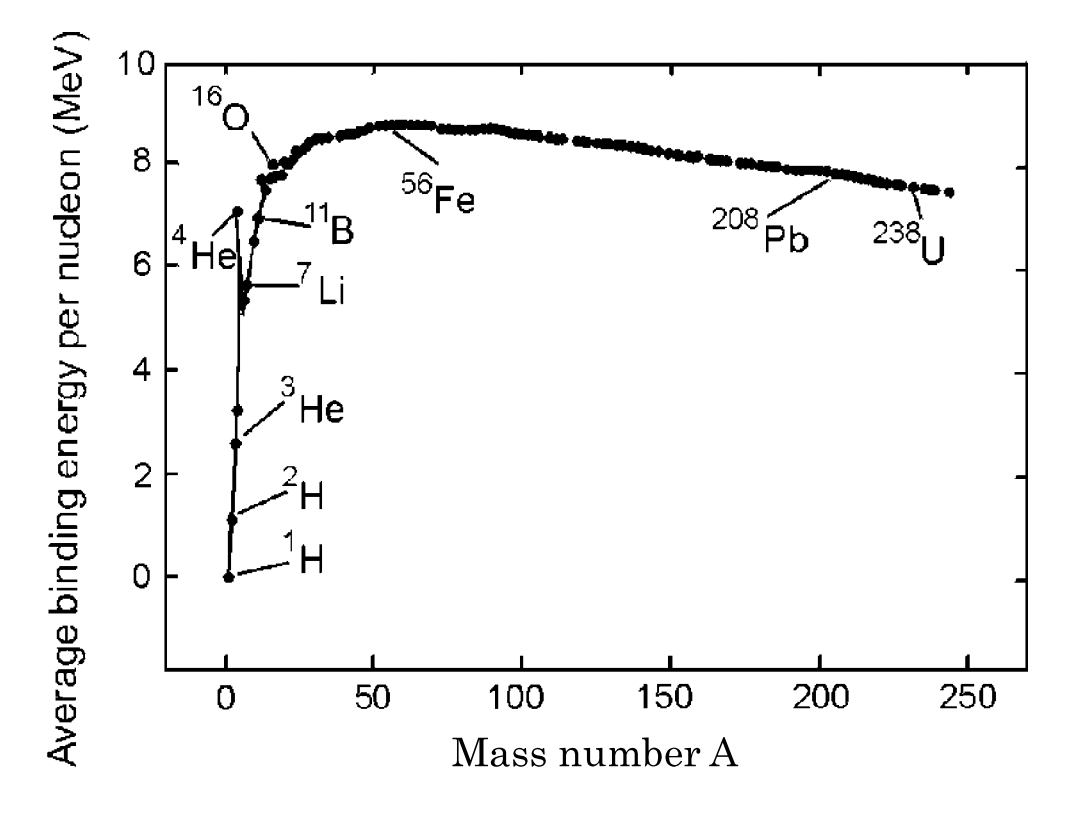
\includegraphics[height = 7cm]{BindingEnergy}
        \\{\tiny Kamal, A. "Nuclear Physics", Berlin : Springer (2014).}
       
    
\end{frame}

%------------------ R-Process 1 ------------------------------------------------------

\begin{frame}{R-Process}

\begin{itemize}
    \item Neutron capture rate``rapid" relative to $\beta$-decay rate.
\end{itemize}

        \centering
        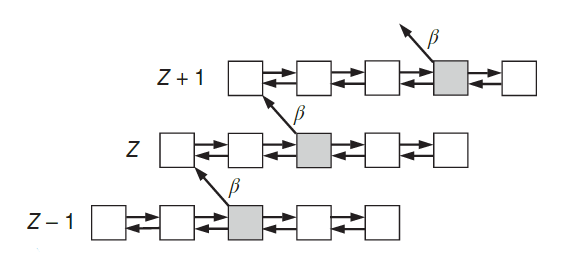
\includegraphics[height=6cm]{isotopicChain2}
        \\{\tiny Iliadis, C. ``Nuclear Physics of Stars", Weinheim, Germany : Springer (2015).}

\end{frame}

%----------------- R-Process 2 -------------------------------------------------------

\begin{frame}{The Problem}

\begin{itemize}
    \item R-Process path wonders very far from stability.
    \item Majority of nuclei never observed.
    \item Very little experimental data on exotic nuclei.
    \item Does shell structure even persist for exotic nuclei?
\end{itemize}

        \centering
        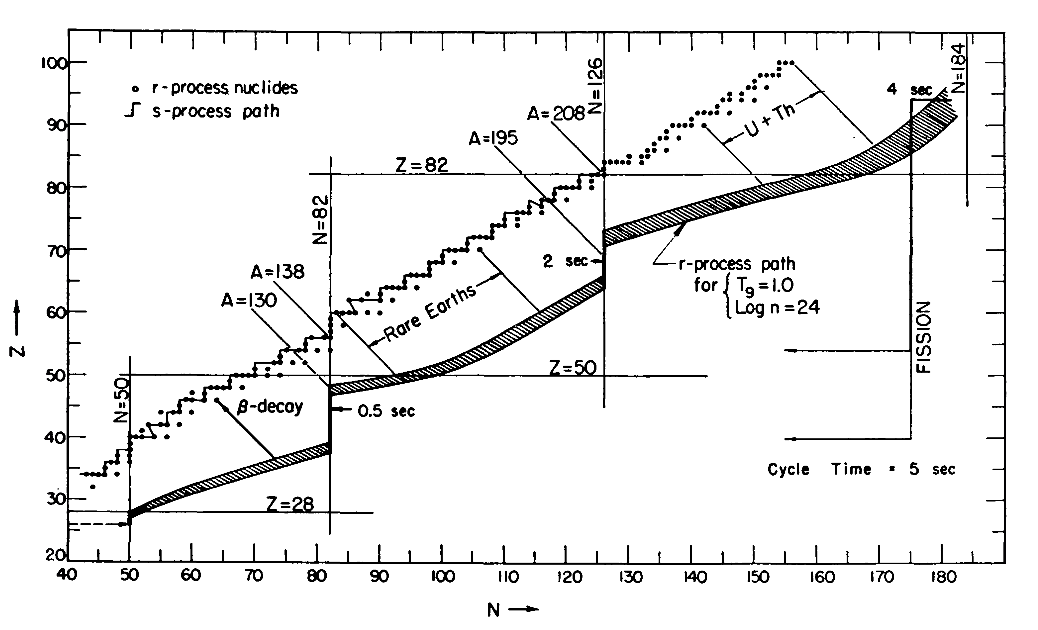
\includegraphics[height = 5.5cm]{RProcessPath}
       \\{\tiny Seeger, P.A., Fowler, W.A., Clayton, D.D. \textit{AstroPhys. J. Suppl} \textbf{11} (1965).}

\end{frame}

%----------------- This Project -------------------------------------------------------

\begin{frame}{This Project}
\begin{itemize}
    \item Analyse data from proton knockout experiments using $^{208}Pb$ and $^{12}C$ targets.
    \item Determine number of protons knocked out per reaction.
    \item Determine masses of residual exotic nuclei.
    \item (Possibly deduce energy level structure.)
\end{itemize}

\end{frame}

%---------------- Proton Knockout at MAMI ---------------------------------------------

\begin{frame}{Proton Knockout At MAMI}
\begin{itemize}
    \item Use electron beam to produce photons by Bremstrahlung and direct onto target.
    \item Photons knockout nucleons via several processes (eg. $\pi^{0}$ production).
    \item Use Crystal Ball detector and Particle Identification Detector (PID) to measure knockout proton energies.
    \item Reconstruct mass of nuclei.
\end{itemize}

    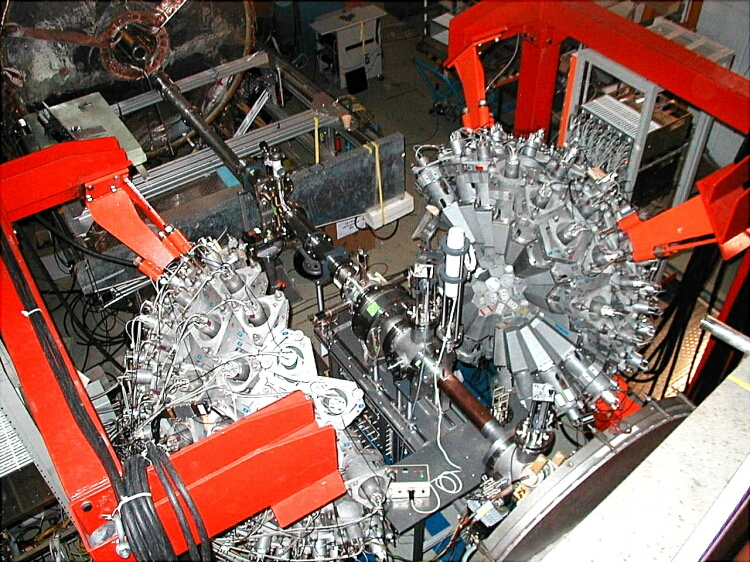
\includegraphics[height = 4cm, right]{openCB}

\end{frame}
%-------------- Data Calibration -------------------------------------------------------

\begin{frame}{Energy Calibration}

\begin{itemize}
    \item Energy lost escaping target, travelling through PID etc.
    \item Use Geant4 Monte-Carlo simulation to model energy losses and calculate corrections.
\end{itemize}

    \centering
    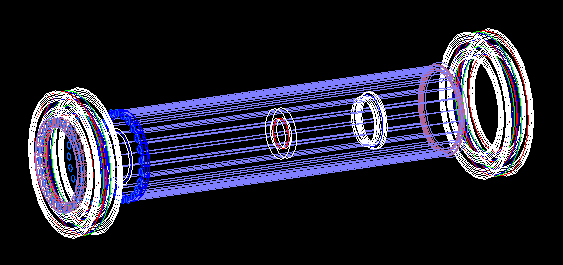
\includegraphics[height= 5cm]{AllIn}

\end{frame}

\end{document}
